\section{Massive Star Evolution}

Stars with an inital mass $>8 M_\odot$ undergo the series of nuclear burning phases described above.
\[
\mathrm{H} \rightarrow \mathrm{He} \rightarrow \mathrm{C} \rightarrow \mathrm{Ne} \rightarrow \mathrm{O} \rightarrow \mathrm{Si} \rightarrow \mathrm{Fe} \rightarrow \text{core collapse}.
\]
These burning phases lead to the structure of the star being separated convective shells with primary burning structures, as seen in Figure \ref{fig:Prialnik_Fig9.19}.
\begin{figure}[!htbp]
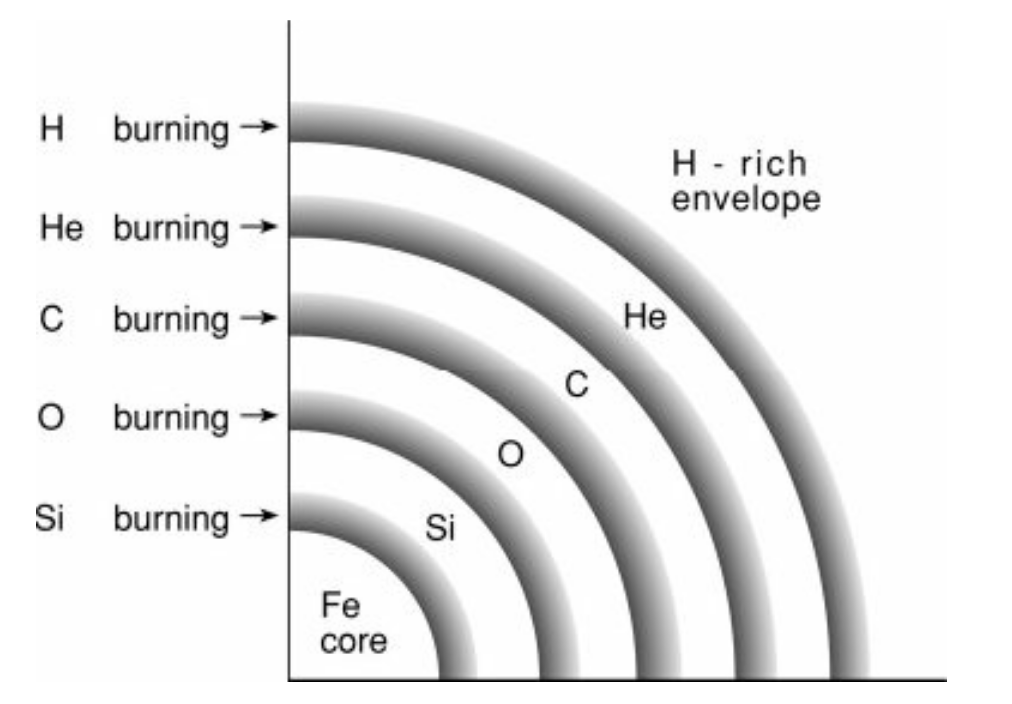
\includegraphics[width=\textwidth]{chapters/1/figures/Prialnik_Fig9.19.png}
\caption{Taken from \cite{prialnikIntroductionTheoryStellar2009} Figure 9.19: Schematic structure of a supernova progenitor star.
\label{fig:Prialnik_Fig9.19}}
\end{figure}

After the formation of the Fe-core and the star begins to rapidly contract as nuclear burning no longer can balance the gravitational force.
This leads to a Type II supernova explosion where further shockwave induced nucleosynthesis can occur \cite{prialnikIntroductionTheoryStellar2009}.
The core of the star leaves behind a neutron star or black hole, and all other material is ejected into the interstellar medium.
The exact location of where mass is ejected from changes the yields of massive star nucleosynthesis as anything under it will remain in the star.
\cite{ritterNuGridStellarData2018} place this mass cut for massive stars around the position of the Si/O-shell.

\subsection{O-C Shell Mergers}

In the final stages of advanced O-shell stellar burning, hours before the core collapse of the star, anywhere from 20\% to 40\% of 1-D massive star models have been found to have a merger of the O-, Ne-, and C-shells \citep{rauscherNucleosynthesisMassiveStars2002, ritterConvectivereactiveNucleosynthesisSc2018, collinsPropertiesConvectiveOxygen2018, robertiGprocessNucleosynthesisCorecollapse2023, robertiOccurrenceImpactCarbonOxygen2025}.
This phenomenon is known as an O-C shell merger.
Figure \ref{fig:kippenhahn_ritter} shows a Kippenhahn diagram of the merger of the O- and C-burning shells for a $15M_\odot$ $Z=0.02$ model from \cite{ritterNuGridStellarData2018}.

\begin{figure}[!htbp]
\includegraphics[width=\textwidth]{chapters/1/figures/Kippenhahn_Ritter+2018.pdf}
\caption{Kippenhahn diagram showing the merger of the convective O and C-burning shells for the $15M_\odot$ $Z=0.02$ model from \cite{ritterNuGridStellarData2018}. The O-burning shell extends from $1.55 M_\odot$ to $1.95 M_\odot$. The first convective C-burning shell sits directly on top from $1.96 M_\odot$ to $2.11 M_\odot$ and additional convective C-burning shells that are subsumed are above. The merger onsets at $\log_{10}(t-t_{\mathrm{end}}) /\mathrm{yr} \approx -3.85$ and reaches full extent at $\approx-4$.
\label{fig:kippenhahn_ritter}}
\end{figure}

These mergers occur when the convective O- and C-shells grow large enough to overlap, forming a single extended convective region.
These mergers are known to have peculiar markers of nucleosynthesis because the convective-reactive environment of the O-shell, such as the production of the odd-Z elements P, Cl, K, and Sc which are underproduced in galactic chemical evolution calculations \citep{ritterConvectivereactiveNucleosynthesisSc2018,robertiOccurrenceImpactCarbonOxygen2025}.
In addition to these isotopes, the O-C shell merger has been a location for the production of the $p$-nuclei \citep{rauscherNucleosynthesisMassiveStars2002, ritterConvectivereactiveNucleosynthesisSc2018, robertiGprocessNucleosynthesisCorecollapse2023}.
As C-shell material containing stable $s$- and $r$-process seeds is ingested into the much hotter O-shell temperatures, they undergo $\gamma$-process.
The O-C shell merger nucleosynthesis has been found to dominate this production independent of the peak energy of the supernova explosion \citep{robertiGprocessNucleosynthesisCorecollapse2024b}. 

O-C shell mergers have also been understood to be important for seeding asymmetries important for the supernova \citep{mullerStatusMultiDimensionalCoreCollapse2016, collinsPropertiesConvectiveOxygen2018, mullerHydrodynamicsCorecollapseSupernovae2020, yadavLargescaleMixingViolent2020a, andrassy3DHydrodynamicSimulations2020}.
The shell mergers are highly asymmetric and provide perturbations necessary for the supernova explosion in the O-shell \citep{collinsPropertiesConvectiveOxygen2018}.